\StartPlate{V05}{The complete cubic corner spectrum}{A finite obstruction can exclude a template without excluding every host.}
\begin{center}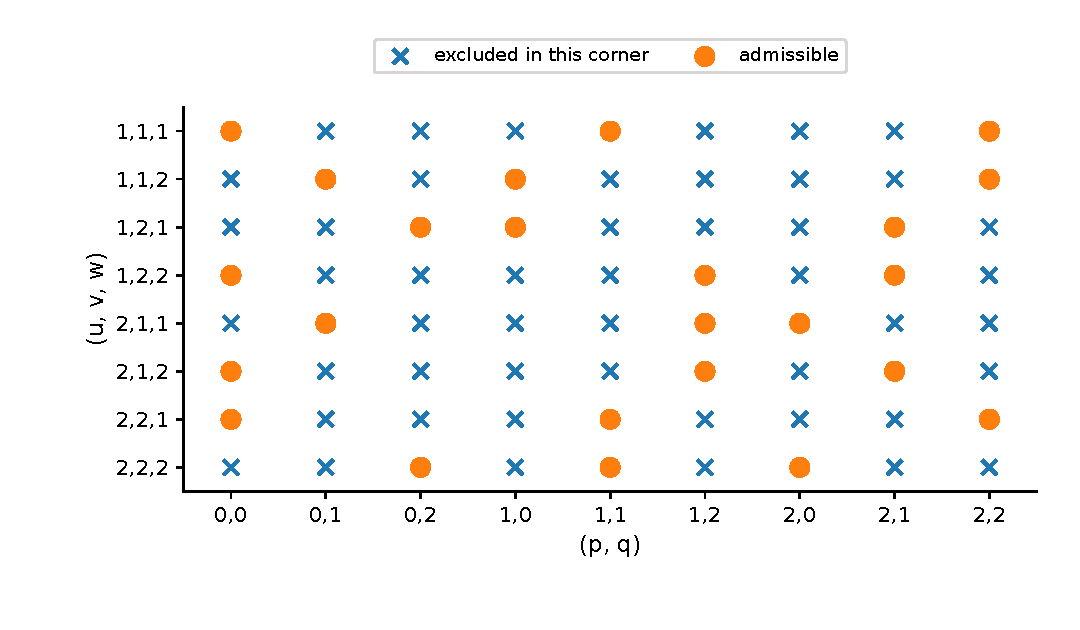
\includegraphics[width=\linewidth]{figures/V05.pdf}\end{center}
Rows run through the eight nonzero triples $(u,v,w)\in\F_3^3$. Columns run through all nine pairs $(p,q)$. A circle marks a solvable target in the specified corner. A cross marks an excluded target.
\[
u=cd,\quad v=ab,\quad w=bc,\quad
p=c(a-h),\quad q=b(d-h).
\]
Elimination gives the exact criterion $p+u=w(q+v)$. Thus precisely $24$ of the $72$ targets are admissible. The data enumerate all five coefficients over $\F_3$ and independently compare their image with this criterion.

The target $(1,1,1,2,2)$ becomes possible when the fifth coefficient $h$ is allowed. The target $(1,1,1,1,2)$ remains impossible. The inherited structural calculation explains why the larger corner has the same decisive leading condition. Its scope is that corner. The later arbitrary-exponent binder changes the construction rather than claiming that this negative result vanished.
\vfill\PlateSource{Exhaustive finite spectrum}{Part II, Section 19.2}{50}
